\documentclass[11pt]{utalcaDoc}
\usepackage{alltt}
\usepackage{underscore}
\usepackage[utf8]{inputenc}
\usepackage[activeacute,spanish]{babel}
\usepackage{verbatim}
\usepackage[pdftex]{graphicx}
\usepackage{ae}
\usepackage{amsmath}
\usepackage{amsfonts}
\usepackage{pdflscape}
\usepackage{inconsolata}
\usepackage{url}
\usepackage{hyperref}
\usepackage{listings}
% \usepackage{placeins}
\usepackage[section]{placeins}
\usepackage[stable]{footmisc}
\usepackage{minted}

\title{{\bf Seguridad Informática}\\ Laboratorio 2}
\author{Erik Regla\\ eregla09@alumnos.utalca.cl}
\date{\today}

\begin{document}
\maketitle
\newpage
\tableofcontents
\newpage

\section{Actividades}
\subsection{Actividad 1}{Instale el cliente de correo Thunderbird según la versión de sistema operativo que posea. Una vez terminada la instalación del cliente de correo, configure su cuenta de correo institucional y haga pruebas de envío y recepción de correo electrónico para comprobar dicha configuración. ¿Durante la instalación y configuración debió aplicar alguna opción o medida de seguridad?}

\begin{minted}{bash}
	#/bin/bash
	## Instalación de thunderbird
	sudo apt install -y thunderbird
\end{minted}

\begin{figure}[ht]
	\centering
	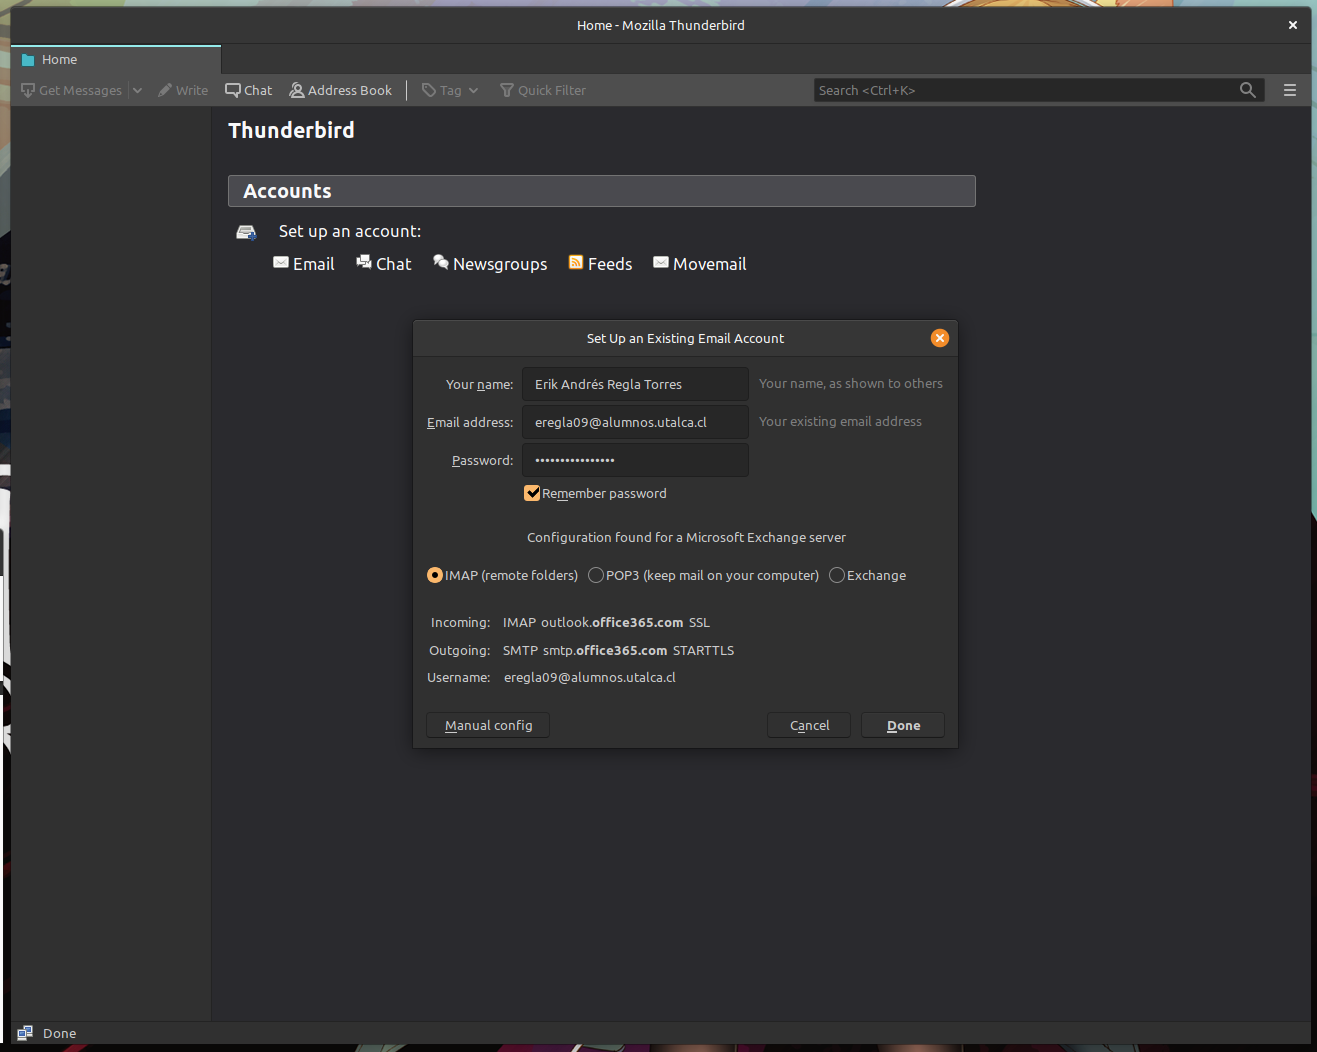
\includegraphics[width=.6\textwidth]{images/thunderbird2}\\
	\caption{Actividad 1: Instalación de thunderbird}
	\label{FIG:thunderbird1}
\end{figure}

\begin{figure}[ht]
	\centering
	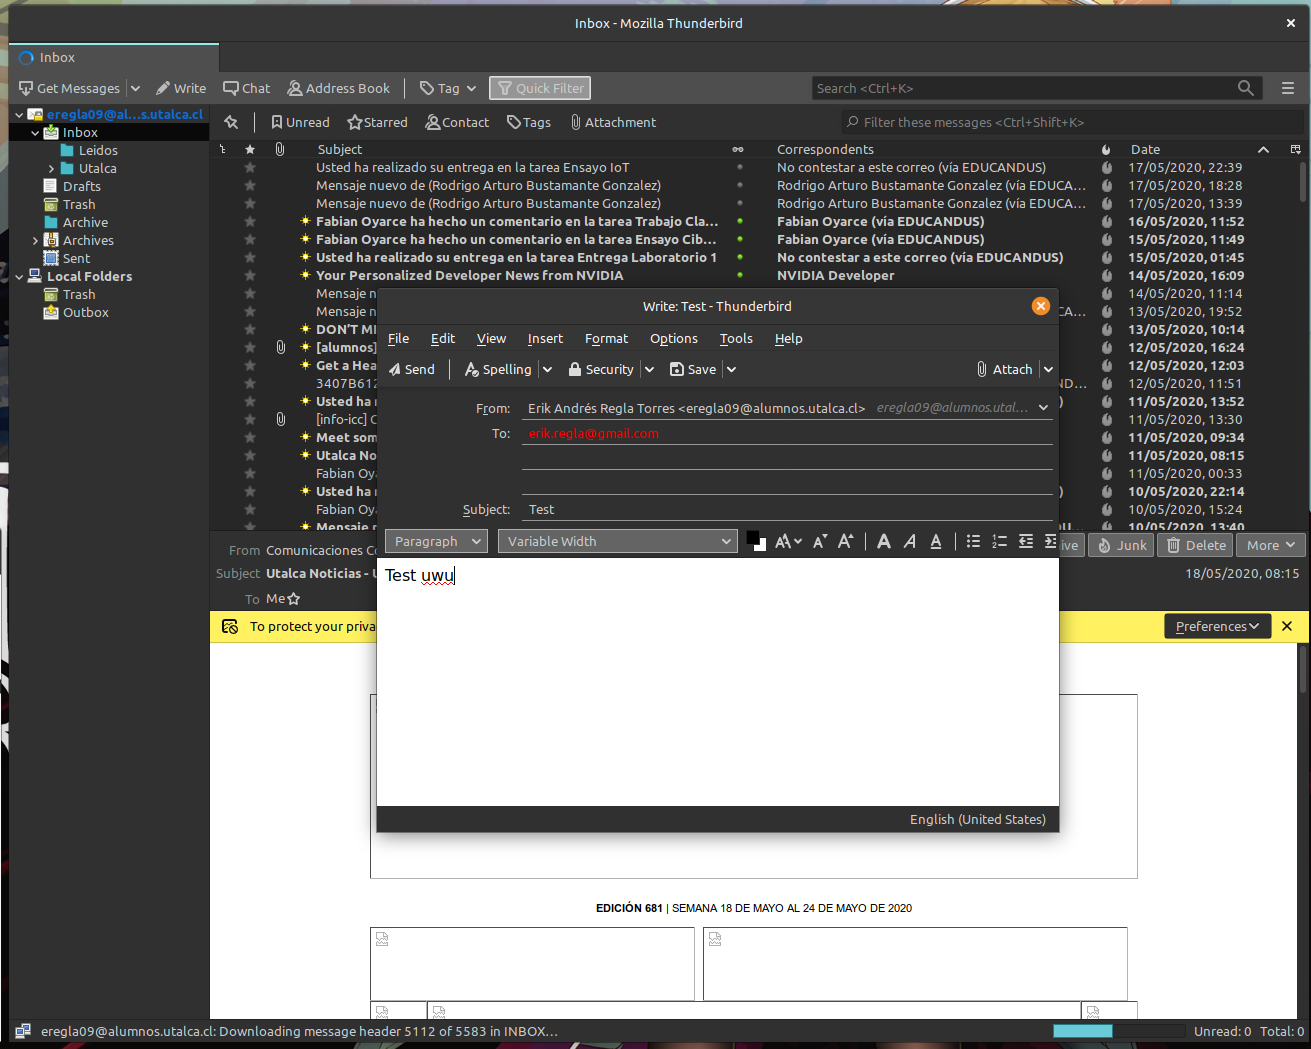
\includegraphics[width=.6\textwidth]{images/thunderbird1}\\
	\caption{Actividad 1: Instalación de thunderbird}
	\label{FIG:thunderbird2}
\end{figure}

\begin{figure}[ht]
	\centering
	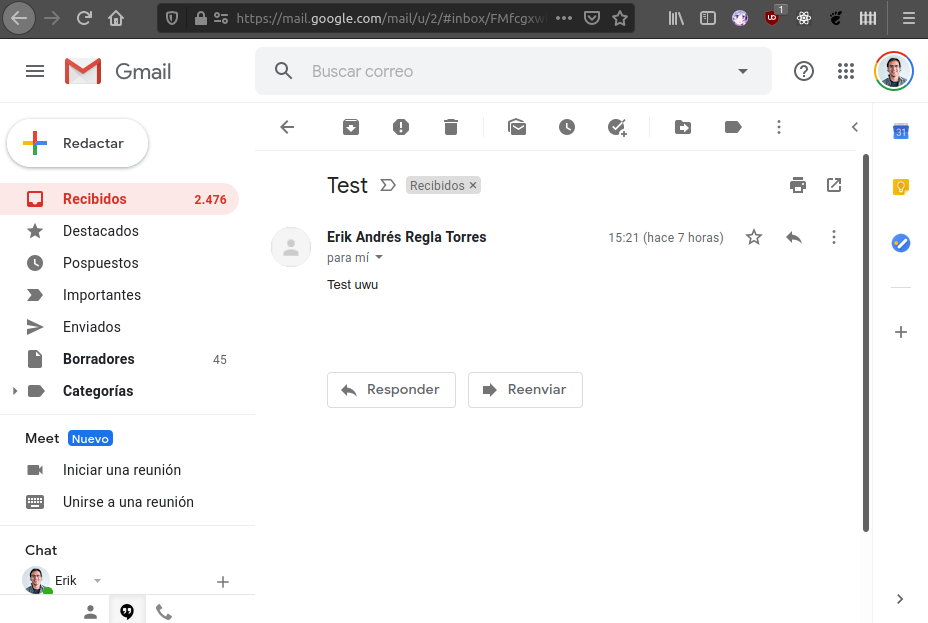
\includegraphics[width=.6\textwidth]{images/gmail1}\\
	\caption{Actividad 1: Lectura de correo enviado a Gmail}
	\label{FIG:thunderbird2}
\end{figure}

Durante la instalación adicionalmente a la contraseña no fue solicitado ningún otro mecanismo de autenticación.

\subsection{Actividad 2}{Una vez configurada y probada su cuenta de correo, aplique las siguientes medidas para mejorar la seguridad y uso del cliente de correo:
Mostrar cuerpo del mensaje como Texto,
Inhabilitar el envío de correo electrónico HTML,
Configurar contraseña maestra,
No permitir contenido remoto en mensajes,
No recordar sitios web y enlaces que haya visitado,
No aceptar cookies de los sitios,
Permitir a los antivirus poner en cuarentena mensajes individuales.
En el informe deberá explicar como cada una de las medidas solicitadas ayudan a mejorar la seguridad y cual es la propiedad que ayuda a mejorar (Integridad, Confidencialidad o Integridad).}


\begin{figure}[ht]
	\centering
	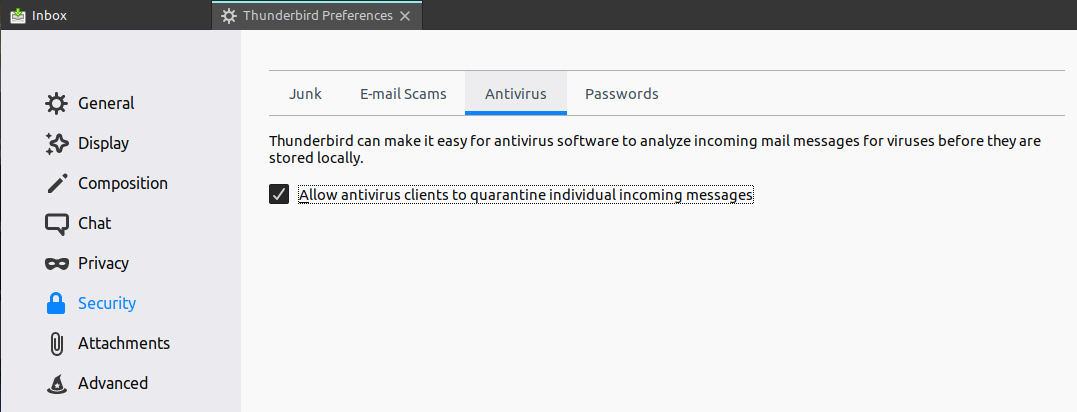
\includegraphics[width=.6\textwidth]{images/seguridad1}\\
	\caption{Actividad 2: Configuración de seguridad de ThunderBird}
	\label{FIG:seguridad1}
\end{figure}

\begin{figure}[ht]
	\centering
	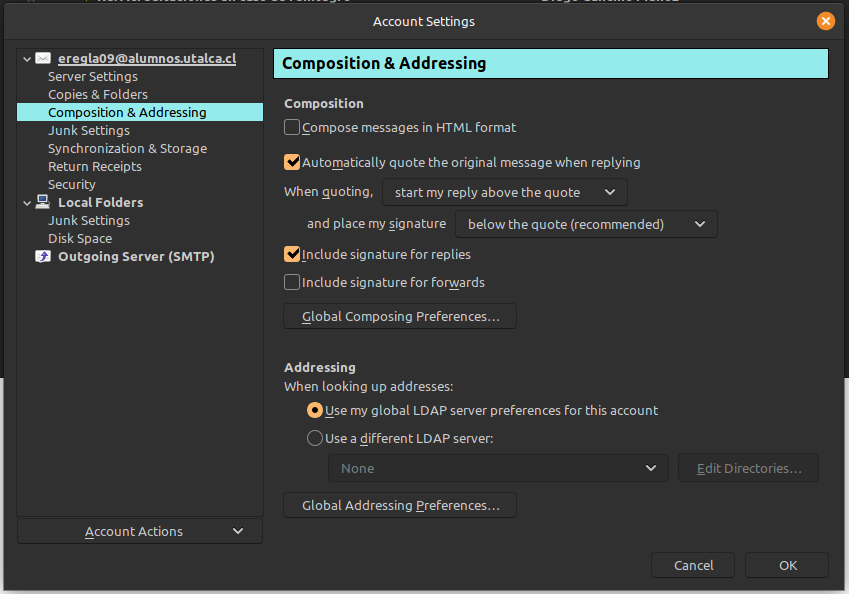
\includegraphics[width=.6\textwidth]{images/seguridad2}\\
	\caption{Actividad 2: Configuración de seguridad de ThunderBird}
	\label{FIG:seguridad2}
\end{figure}

\begin{figure}[ht]
	\centering
	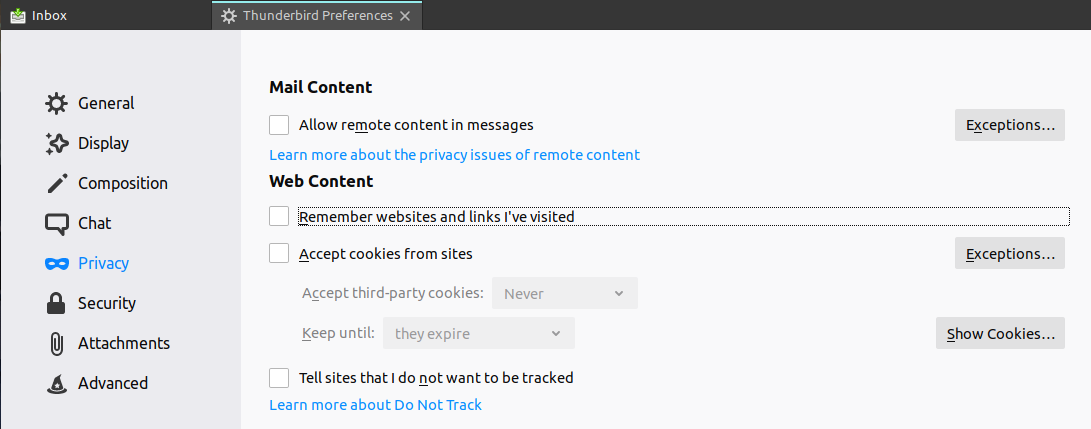
\includegraphics[width=.6\textwidth]{images/seguridad3}\\
	\caption{Actividad 2: Configuración de seguridad de ThunderBird}
	\label{FIG:seguridad3}
\end{figure}

Efectos en la integridad, confidencialidad y disponibilidad\footnote{La cual está mal escrita en el enunciado}:
\begin{itemize}
	\item \textbf{Mostrar cuerpo del mensaje como Texto:} La visualización del correo se lleva a cabo en navegadores, los cuales podrían contener enlaces maliciosos ocultos dentro de el texto bajo tipografias similares, ejecución de scripts, etc.
	\item \textbf{Inhabilitar el envío de correo electrónico HTML:} Idem a la anterior pero en el caso del envío, a modo de proteger a nuestro destinatario y su disponibilidad del servicio.
	\item \textbf{Configurar contraseña maestra:} Permite almacenar las contraseñas por medio de un llavero, el cual \textit{teoricamente} solo funciona dentro de la misma máquina donde este se creó (en la práctica no es el caso), de este modo evita la escritura manual de contraseñas. Arma de doble filo.
	\item \textbf{No permitir contenido remoto en mensajes:} Permite mantener una lectura confidencial del correo al evitar el uso de trackers como \textit{pixeles}.
	\item \textbf{No recordar sitios web y enlaces que haya visitado:} Previene la obtención de historiales desde el navegador integrado al lector de correo para proteger la confidencialidad del usuario.
	\item \textbf{No aceptar cookies de los sitios:} Idem a la anterior pero con las cookies almacenadas.
	\item \textbf{Permitir a los antivirus poner en cuarentena mensajes individuales:} En el caso que algun mensaje pueda tener contenido malicioso permite que una heramienta externa pueda aislarlo, protegiendo la disponibilidad de los demás mensajes de manera individual como la de la aplicación (obviamente cubre todos los aspectos y solo funciona si tienes antivirus).
\end{itemize}

\subsection{Actividad 3}{Utilice el cliente de correo Thunderbird y el complemento Enigmail para Thunderbird para realizar el envío de correo firmado y cifrado. Utilice la cuenta de correo de alumno para configurar su set de claves y envíe su clave pública a robustamante@utalca.cl. Nota: Necesitará la clave pública del correo robustamante@utalca.cl, la cual deberá solicitar durante la realización de la práctica.}



\begin{figure}[ht]
	\centering
	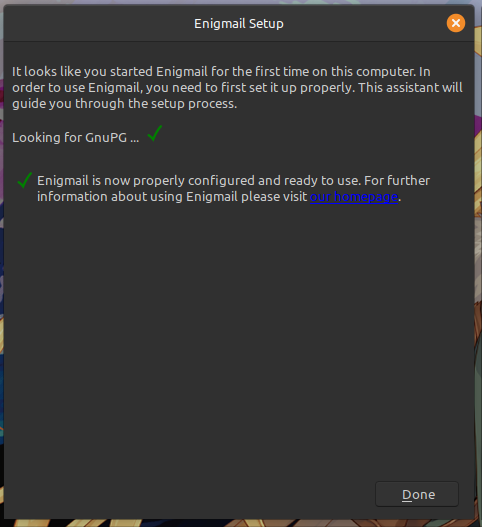
\includegraphics[width=.6\textwidth]{images/send1}\\
	\caption{Actividad 3: Envío de llave pública}
	\label{FIG:send1}
\end{figure}

\begin{figure}[ht]
	\centering
	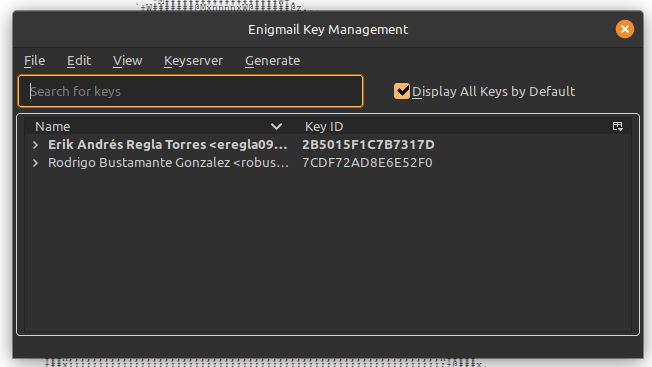
\includegraphics[width=.6\textwidth]{images/send2}\\
	\caption{Actividad 3: Envío de llave pública}
	\label{FIG:send2}
\end{figure}

\begin{figure}[ht]
	\centering
	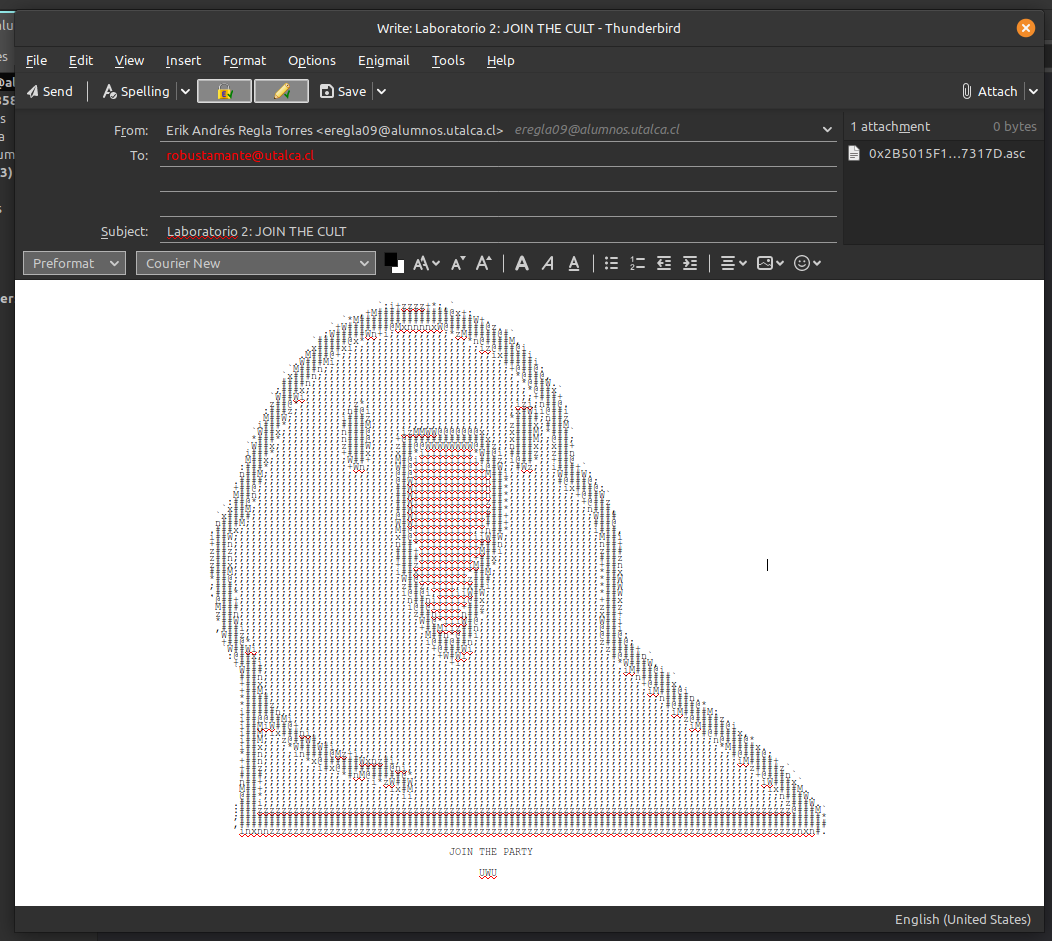
\includegraphics[width=.6\textwidth]{images/send3}\\
	\caption{Actividad 3: Envío de llave pública}
	\label{FIG:send2}
\end{figure}

\subsection{Actividad 4}{Además, deberá investigar qué es y como funciona PGP, dando énfasis en porqué es importante utilizarlo y como piensa que ayuda a la Confidencialidad, Integridad y Disponibilidad.}

La encripción PGP se basa en el \textit{protocolo de llave pública}, en la cual cada contraparte contiene fragmentos de la llave del destinatario, permitiendole cifrar el contenido. Una forma de visualizar este proceso es con la analogía del cofre y la llave. Supongamos que deseamos enviar una carta de una persona a otra, pero no queremos que nadie mas lea esta. La condicion inicial es que toda transferencia pasa por un tercero, quien puede leer el mensaje. Entonces, nuestro destinatario nos entrega un cofre abierto (la llave pública) que utilizamos para almacenar nuestra carta y luego cerramos el cofre (cifrado con llave pública). Luego enviamos el cofre el cual nadie es capaz de abrir (ya que nadie tiene la llave) y una vez llega al destinatario este puede abrir el cofre utilizando la llave que solo el posee (llave privada) y leer la carta (leer el mensaje).


\begin{figure}[ht]
	\centering
	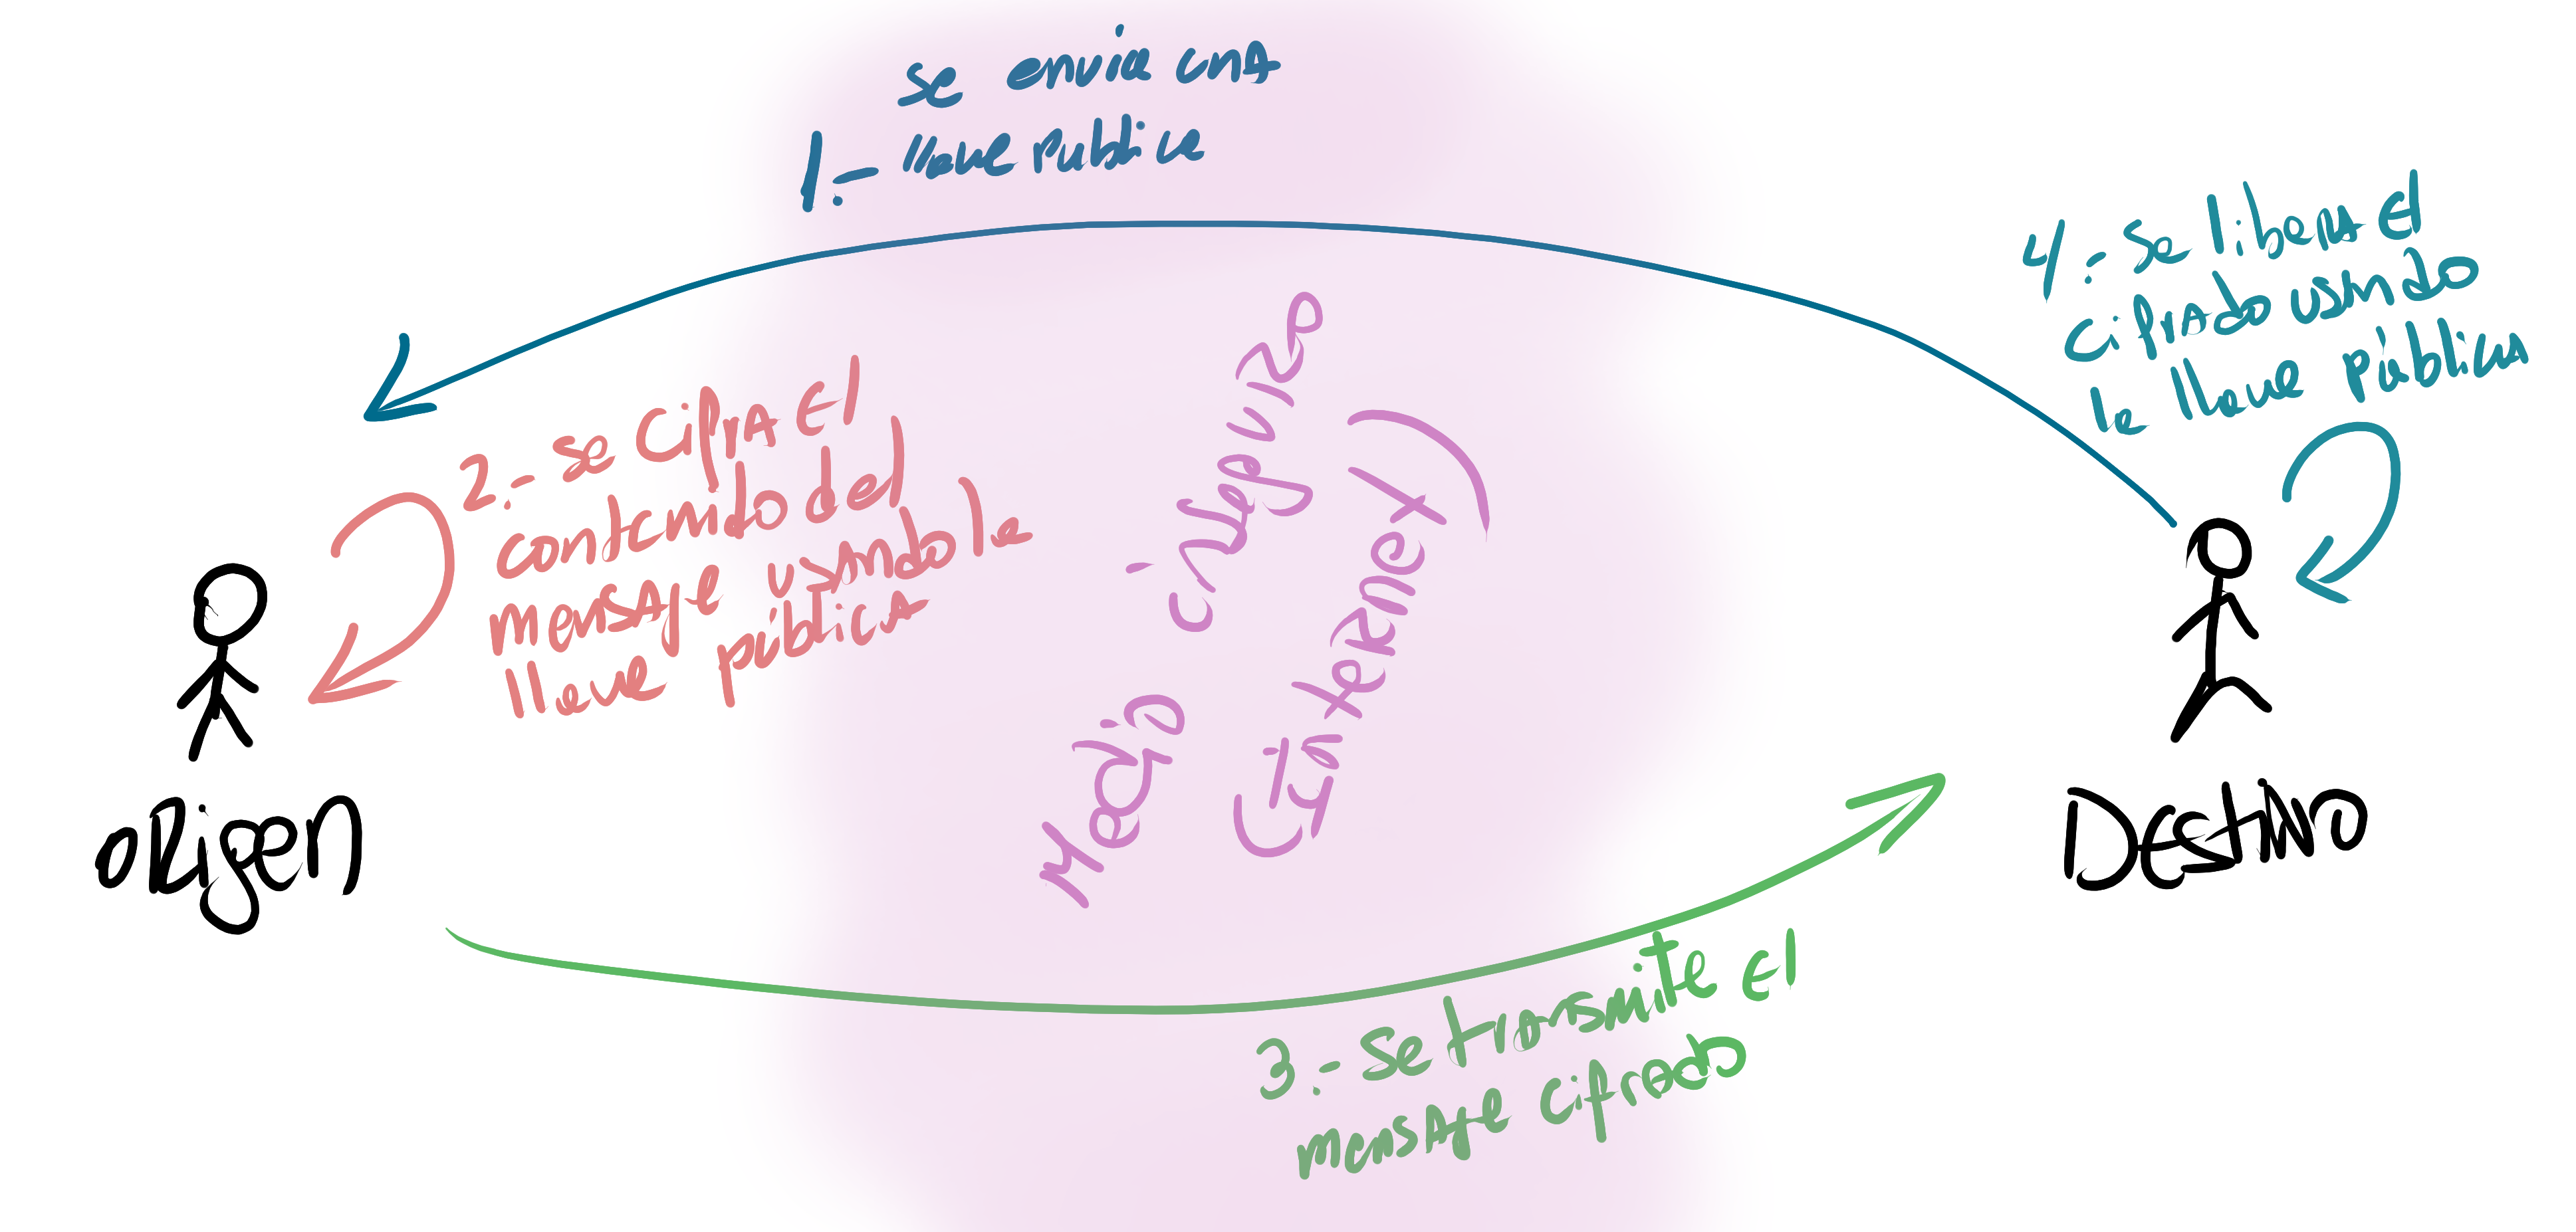
\includegraphics[width=.8\textwidth]{images/pgp}\\
	\caption{Actividad 4: Caricaturización de como funciona PGP}
	\label{FIG:caricatura}
\end{figure}

Para que este proceso pueda funcionar, es previo necesario intercambiar llaves públicas. ESto ayuda a mantener la confidencialidad del mensaje ya que si la llave pública es capturada por un tercero, su único uso es cifrar mensajes para que los pueda leer un tercero, esta llave per se no es capaz de decriptar información alguna \textit{en teoría}.\cite{REF:pgp}

Sin embargo este método no está libre de vulnerabilidades, como por ejemplo ataques de exfiltración, los cuales abusan del contenido activo de un documento HTML para poder exfiltrar contenido por medio de los enlaces que este puede contener\cite{REF:efail}. Sin embargo este tipo de ataques no afecta directamente a PGP, si no mas bien a los clientes involucrados en el manejo de este y las practicas derivadas del mismo. No es como si fuera a ser final de PGP\cite{REF:hackaday}.
% \subsection{Actividad 1}{¿Qué residuo y trama a enviar se obtiene al dividir $x^7 + x^5 + 1$ y el polinomio generador $x3 + 1?$}
% Refiérase a la figura \ref{FIG:resolucion1} en la página \pageref{FIG:resolucion1}.
% \begin{figure}[ht]
% 	\centering
% 	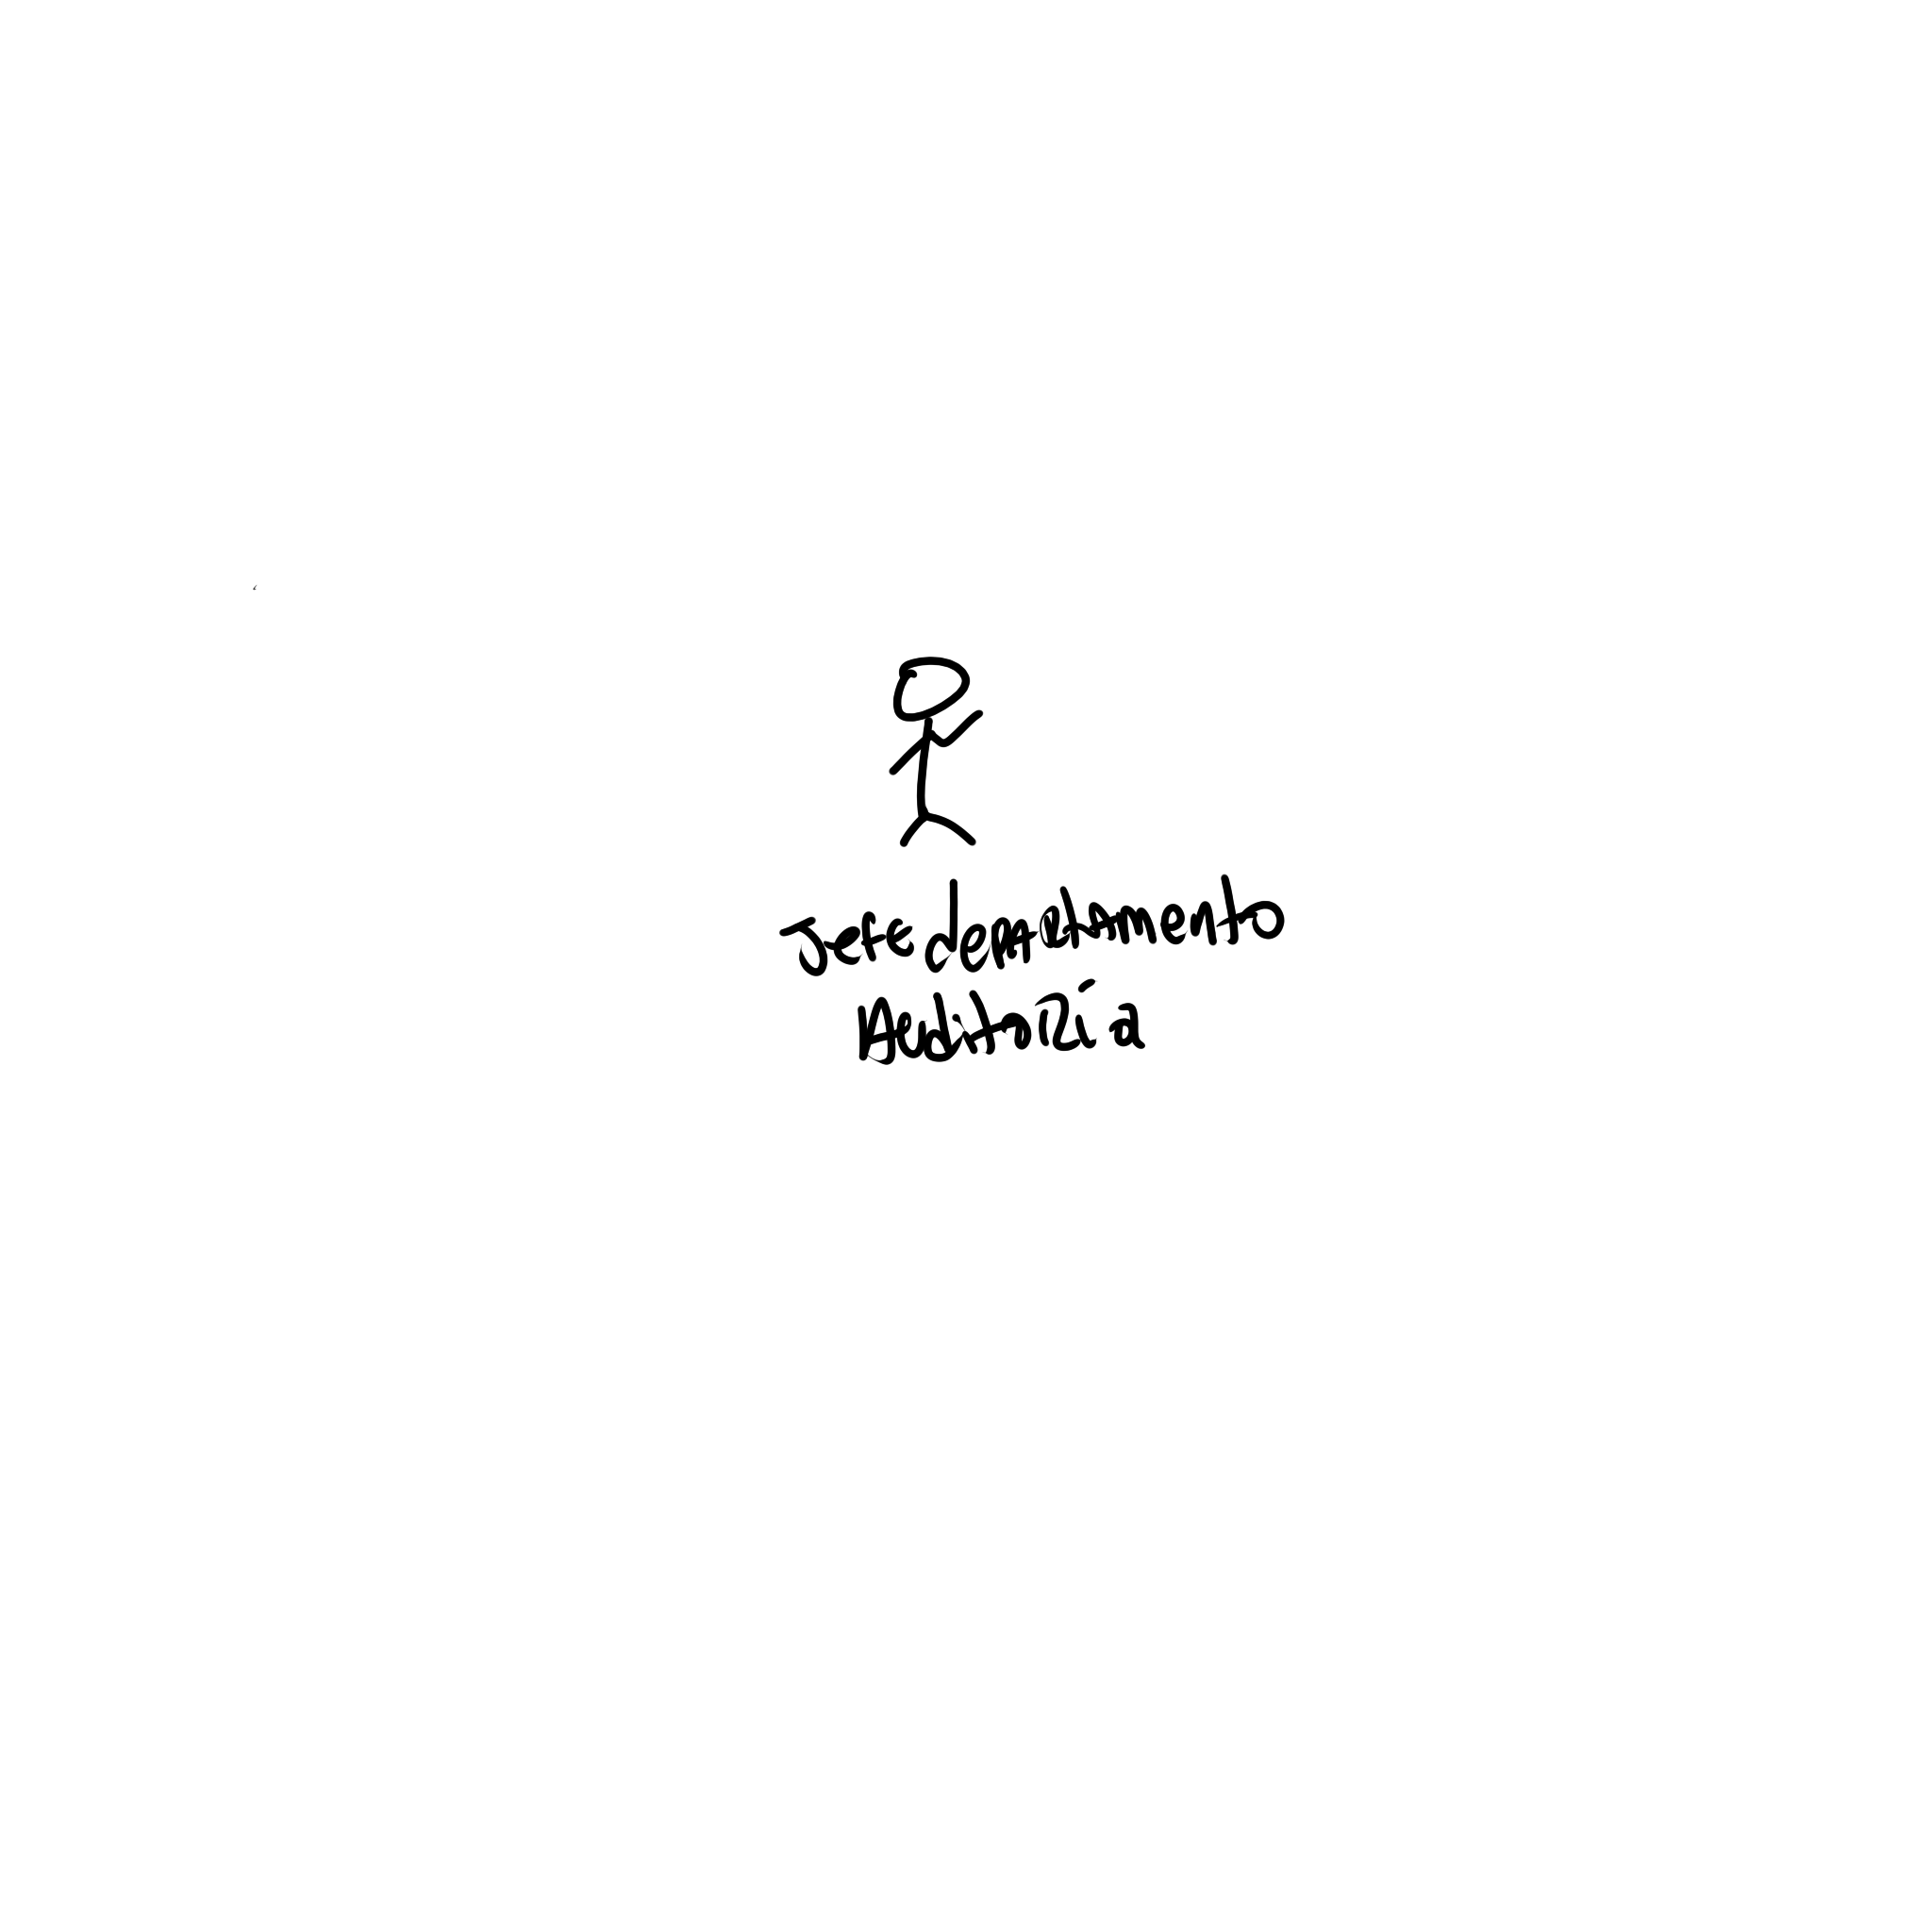
\includegraphics[height=.6\textheight]{images/1}\\
% 	\caption{Resolución 1}
% 	\label{FIG:resolucion1}
% \end{figure}


\begin{thebibliography}{9}
	\bibitem{REF:pgp}
	GnuPG Homepage.
	\textit{Documentation}.
	https://gnupg.org/faq/gnupg-faq.html.


	\bibitem{REF:efail}
	eFail.de Homepage.
	\textit{Homepage}.
	https://efail.de.


	\bibitem{REF:hackaday}
	Hackaday.
	\textit{Explaining Efail And Why It Isn’t The End Of Email Privacy}.
	https://hackaday.com/2018/05/21/explaining-efail-and-why-it-isnt-the-end-of-email-privacy/.
\end{thebibliography}

\end{document}